% THIS IS ICT4S_PROC.TEX - VERSION 1.0 based on SIGPROC_SP.TEX (ACM SIG Proceedings Latex format)
% WORKS WITH V1 OF ICT4S_PROC_ARTICLE.CLS based on ACM_PROC_ARTICLE_SP.CLS V3.2SP
% August 2012
%
% It is an example file showing how to format the full paper for the ICT4S 2013 conference proceedings
%
% LaTeX2e document class file for Conference Proceedings submissions.
% ----------------------------------------------------------------------------------------------------------------
% ---------------------------------------------------------------------------------------------------------------
% It is an example which *does* use the .bib file (from which the .bbl file
% is produced).
%
% For tracking purposes - this is based on sigproc-sp V3.1SP - APRIL 2009


% NOTE ON THE DIFFERENCES:
% We have slightly tweaked the .cls and the .tex to allow a result similar to the 
% Word template provided for the ICT4S 2013.
% Authors:
% - below the title the authors are given as a centered list with footnote-like 
%   marks pointing to affiliations  (use \amarks{<number>} )
% - below the list of authors follows a list of addresses 
%     *each starting on a new line
%     *explaining one of the marks used in the list of authors
% - each address consists of the affiliation followed by the email addresses of the
%   authors belonging to the affiliation, an empty line before each affiliation
% - One email per author suffices
% 

\newcommand{\amark}[1]{\raisebox{5pt}{\small $#1$}}

\documentclass{ict4s_proc_article}
\usepackage{cite}
\usepackage{url}

\begin{document}

\title{Makahiki+WattDepot: An open source software stack for 
next generation energy research and education}

%
% You need the command \numberofauthors to handle the 'placement
% and alignment' of the authors beneath the title.
%
% Do not use the \alignauthor commands.

\numberofauthors{5} % necessary for working with the adapted style

\author{
% precede each author name, affiliation/snail-mail address and
% e-mail address. Additionally, tag each line of
% affiliation/address with \affaddr, and tag the
% e-mail address with \email.
%
 Philip M. Johnson, 
 Yongwen Xu,
 Robert S. Brewer,
 George E. Lee,
 Andrea Connell \\
 \\ % an empty line before each new affiliation
       \affaddr{Collaborative Software Development Laboratory, University of Hawaii at Manoa, Honolulu, HI 96822 USA}\\
\email{johnson@hawaii.edu, yxu@hawaii.edu, rbrewer@hawaii.edu, gelee@hawaii.edu, connell4@hawaii.edu}\\
}

\date{19 August 2012}

% The editor remark on the first page at the bottom of the first column 
% is necessary!
\editorremark{
\hrule\par\rule[-0.65em]{0pt}{0em}\\
ICT4S 2013: Proceedings of the First International Conference on
Information and Communication Technologies for Sustainability, ETH Zurich, 
February 14-16, 2013. Edited by Lorenz M.~Hilty, Bernard Aebischer, G{\"o}ran Andersson and Wolfgang Lohmann.\\ \noindent http://e-collection.library.ethz.ch} %%W

\maketitle
\begin{abstract}
The accelerating world-wide growth in demand for energy has led to the conceptualization
of a ``smart grid'', where a variety of decentralized, intermittent, renewable energy
sources (for example, wind, solar, and wave) would provide most or all of the power
required by small-scale ``micro-grids'' servicing hundreds to thousands of consumers. Such
a smart grid will require consumers to transition from passive to active participation in
order to optimize the efficiency and effectiveness of the grid's electrical capabilities. 
This paper presents a software stack called comprised of two open source software systems,
Makahiki and WattDepot, which together are designed to engage consumers in energy issues
through a combination of education, real-time feedback, incentives, and game mechanics. We
detail the novel features of Makahiki and WattDepot, along with our initial experiences using
them to implement an energy challenge called the Kukui Cup.

\end{abstract}

%NO Categories 
%NO Terms

\keywords{smart grid, energy research, open source, game engine, energy repositories}

\chapter{Introduction}
Delivering high quality software products within the budget and in time is the main goal and the most 
challenging task of Software Engineering. Years of scientific research in this area resulted in a 
number of software processes providing detailed guidelines on how to reach 
the goal efficiently. These processes manifested themselfs as the means for improvements in terms 
of quality, speed and cost over existing practices. Many were implemented and tested within academic 
and industrial settings and proved proposed superiority. Some of these processes were successfully 
adopted and standardized in industry shaping the best practices of contemporary software development 
\cite{citeulike:9962021}. Moreover, there are plethora of processes for improving existing processes 
of software development on the team \cite{citeulike:9962027} and personal 
levels \cite{citeulike:9962022}.

The processes I am mentioning here are the well-known large formal models such as Waterfall and Spiral, 
as well as more flexible iterative agile approaches like XP, SCRUM or FDD. These are also sets of 
rules and recommendations which can be applied to certain stages of the software processes 
such as Test Driven Development or Pair Programming; there are general guidelines helping 
to improve the correctness of a product and standards, like CMMI or ISO 9000; guidlines for testing 
and measurements, code syntax rules and formatting styles, code comments 
recomendations \cite{citeulike:900855}. 

From the first sight, taking all this in account,  one would guess that 
the area of software processes is thoroughly explored and there are clear choices of processes 
and models for the one in charge making decision... But it is not true - despite many choices 
one can make, no one can foretell what is the ``best'' process to choose for certain constraints.
What managers are left with are the equal alternatives and vague promises. 
This deficiency in knowledge is the main coause of the ``software crisis'' phenomena point is supported by the fact that according to ``Chaos Report'' from the Standish 
Group (Rubinstein) \cite{SDTimes} only ``35\% of software projects in 2006 can be categorized as successful - meaning 
they were completed on time, on budget and met user requirements''. 
These thirty five percent of success clearly saying that it is somewhat difficult to make 
a statement that we are fully understand and able to control software processes. 
Moreover, over years, while this idea of a software process formalizations shaped the 
programming practices, which once thought to be a creative human activity accessible by amateurs 
and hobbyists \cite{citeulike:9958822} into a serious engineering discipline, bounded 
by requirements for education, standardized processes, rules, certifications, and strict 
financial requirements from stakeholders the opposite idea was born - the idea of 
software development as a craft. Interesting that such a duality of views can be found 
in the work of a single person \cite{citeulike:5203446}.

Clearly, there is a great room for research and improvement of our understanding of software processes.
This exploratory study is yet another attempt at the understanding. In my research work I am 
exploring techniques aiming the understanding of small processes which are 
rather the reflection of personal behaviors or habits of software development rather than a 
formalized constructs. Also, I would like to emphasize, that in this work I will not 
address the need and means of the process synthesis, its quality assessment, productiveness
or any topics related to the software product itself; I would rather focus on the specific issue - 
uncovering an existence and studying the programming habits. 

This thesis presents a methodology for finding recurrent behaviors through the 
analysis of the variety of software process artifacts left after performing a 
software process. I have called this methodology ``Software Trajectory'' and it consists 
of four distinct steps. Each of these steps has a specific goal and compromising variety of 
means to reach it. 
At first software process artifacts are identified and collected. 
At second, they are cleaned, organized and classified. 
On the third step particular research questions are formulated and data are organized and indexed. 
And finally, a set of KDD techniques is applied in order to undercover recurrent behaviors which 
could potentially shed a light on the performed process details. 

My personal motivation for performing this work is coming from the recognition of the 
importance of the software in our lives and the severity of issues with its development. 
Through my everyday experiences with software development and use I have stumble upon 
a number of issues which made me realize that mentioned ``software crisis'' phenomena is very real.
As a user in industrial and academic settings I often find myself facing software failures 
which create numerous difficulties for reaching production or research goals. As a developer, 
in an attempt to be productive and in order to deliver a better software I have studied and 
explored a number of formal processes, however, sometime I found myself seeing a very little of 
rationale behind their application, and moreover, in this exploration, when facing the process
application failing to help I was unable to comprehend what exactly went wrong and what need 
to be changed. All of these experiences made me studying software process research and exploring
novel approaches to software process recovery on my own in order to understand software process better.

\section{Research area overview}
As mentioned above, in this thesis I am focusing on a very narrow subject - exploring approaches
for uncovering of recurrent behaviors or ``programming habits'' out of software process artifacts.
Before narrowing further 


Software is usually coded by teams. Members of these teams are agreed and bound to use 
a particular technologies and development tools, they also agree on following well defined 
development process which is constrained by a timeline and budget. These are necessary 
constraints to keep work organized, however there is a great freedom in what they actually 
do in every single moment of time in order to progress towards lines of code which eventually 
will result in software. For example one developer may follow test first process while
another writes tests at last.  This freedom of choice in ordering of development activities 
while being much appreciated by talented and creative individuals creates an impression 
of chaotic and unordered activities for random observers, newbies and people in 
charge - so there we have all the attempts of imposing an order 
(or control) on all of the development activities. Metrics and models of processes






\section{WattDepot}

Software for energy collection, storage, and analysis tends to come in two flavors that support two ends of the scalability spectrum.  At one end are utility-scale SCADA systems and protocols which are intended to manage macro-grid data \cite{SmartEnergy2.0, OSHAN, OpenPDC}.  At the other end are ``personal scale'' systems such as those provided by energy meter or solar panel manufacturers which are intended to manage information about single households \cite{TED, EMS100}.  We designed WattDepot to support a middle ground that we refer to as ``enterprise-level'' energy management, in which data concerning energy production and consumption of hundreds to thousands of households can be usefully managed~\cite{csdl2-10-05}. Figure \ref{fig:wattdepot} illustrates the architecture of the system, where WattDepot sensors send data from meters attached to energy devices to a server, which can then be queried by clients to provide visualizations and analyses.

\begin{figure}
\begin{center}
\epsfig{file=wattdepot-architecture, width=3in}
\end{center}
\caption{Architecture of WattDepot}
\label{fig:wattdepot}
\end{figure}

Our use of WattDepot has led to a novel set of capabilities to support this middle ground.

\subsection{Meter Agnostic}

Unlike personal-scale systems that are typically tied to a particular manufacturer's product, WattDepot is agnostic about the kinds of meters used to monitor energy production and consumption data, and whether the data is personal-scale or utility-scale. It provides a REST protocol for data transmission that can be used to implement clients for a wide variety of devices; the major constraint is that these devices need to have network access. WattDepot clients can be written in any language that supports the HTTP protocol. We provide a high-level client libraries for Java and JavaScript.

Due to the architectural decoupling of data collection from the rest of the system, WattDepot can be effectively used for simulation and what-if scenario development. This flexibility makes it appropriate as a kind of technological ``scaffolding'' for smart grid applications, where WattDepot can provide clients with simulated production and consumption data early in development, with the simulated data transitioning to live data as these sources go online later in development.

\subsection{Source Aggregation}

WattDepot can represent aggregations of power sou\-rces. For example, a building might have multiple meters monitoring energy consumption, one per floor. WattDepot can represent the power consumed by individual floors, as well as an aggregate source representing the building as a whole. Aggregations can be nested, so that floors can be aggregated into buildings, buildings into neighborhoods, and neighborhoods into cities. It is quite common for the level of abstraction desired by client developers and end users (such as a floor of a building) to actually consist of multiple meters. By providing this aggregation of sources at the server level, client development becomes easier.

\subsection{Data Interpolation}

WattDepot automatically performs data interpolation when necessary. For example, a meter might provide a snapshot of energy usage once per hour for a given device. Clients can request the power consumed by this device at any time instant, and WattDepot will automatically provide interpolation when the requested time does not match a time for which actual sensor data is available. This is essential for the common case where meters do not have perfectly synchronized clocks and are not polled simultaneously, and when making use of the source aggregations discussed in the previous section.

\subsection{Flexible Data Storage}

WattDepot is architecturally decoupled from the underlying data storage technology. This decoupling supports experimentation with both traditional relational as well as NoSQL technologies, and facilitates scalability. Currently, WattDepot implements support for Derby, PostgreSQL, and BerkeleyDB storage systems. Administrators looking for simplicity may opt for the embedded Derby database, while those looking to integrate with existing database infrastructure might decide to use PostgreSQL for data storage.

WattDepot also implements support for ``ephemeral'' data. In some application scenarios, it is useful to send energy data to the WattDepot server quite frequently (i.e. every few seconds) so that clients can monitor current energy consumption with low latency. However, that rate of data sampling is not necessary for historical analyses, which may only require energy data sampling at the rate of every few minutes. WattDepot supports this situation through ephemeral data, which creates an in-memory window during which all recently received energy data is available for retrieval, but stored in the repository only at a much lower sampling rate.

\subsection{WattDepot in the Cloud}

In addition to installation on a local server, WattDepot has been designed to support cloud hosting, sometimes referred to as Platform-as-a-Service (PaaS). In particular, WattDepot can be deployed on the Heroku \cite {HerokuHomePage} cloud-based hosting service. The Heroku PaaS solution allows users to deploy the system and start collecting data without the requirement of server hardware, and Heroku offers flexible capacity depending on the expected workload.

\subsection{Beyond WattDepot}

While WattDepot provides the software infrastructure to collect, store, and analyze energy data, ensuring that the data is collected reliably and accurately reflects reality requires additional effort. As an example, we will examine the steps required to collect data on electricity use in a building. First, the administrator should work with manager of the building to understand the electrical infrastructure: how is power distributed in the building, and how does the distribution relate to the goals to be accomplished through measurement? If electricity is to be monitored at the per-floor level, do the distribution panels match that segmentation?

If the building does not have meters already installed, the administrator will need to select a meter vendor and acquire the meters. The meters will typically need to be installed by licensed electricians. The administrator will need to verify that the installation was performed correctly by checking whether the received data agrees with the expected amount of usage. To allow WattDepot to collect data, reliable network connectivity must be provided for the meters. The meters will also need to be configured to support remote data collection.

If the building already has meters installed, the administrator will need to confirm that the meters are configured correctly and that the data they produce  is sane. When working with existing meter infrastructure, the WattDepot administrator may not have administrative access to the meters, so any configuration changes required may need to be requested from the meter administrator.

Once data collection has been established, the WattDepot administrator will need to establish monitoring of the meters and WattDepot infrastructure so that hardware or software faults can be detected and corrected before they lead to excessive loss of data. By understanding these issues, administrators can ensure that systems built on top of WattDepot receive accurate energy data at appropriate levels of abstraction.


\section{Makahiki}
The feature set of WattDepot creates attractive infrastructure for management of energy data, but research suggests that effective participation of consumers in a next generation smart grid requires more than simple feedback to consumers about their consumption, particularly given the passive nature of their involvement for the past 100 years.

The second component of our open source software stack, Makahiki, represents research intended to create synergy between the need to create knowledge and engagement regarding energy and the ability of so-called ``serious game'' techniques and energy feedback to create participation and engagement \cite{Deterding2011mt,darby-review-2006,Faruqui09,petersen-dorm-energy-reduction}. In Makahiki, online game mechanics are employed with the goal of affecting real-world energy behaviors.  The ultimate goal is to not just affect energy behaviors during the course of the game, but to produce long lasting, sustained change in energy behaviors and outlooks by participants. Figure \ref{fig:makahiki-architecture} illustrates the architecture of Makahiki.

\begin{figure}
\begin{center}
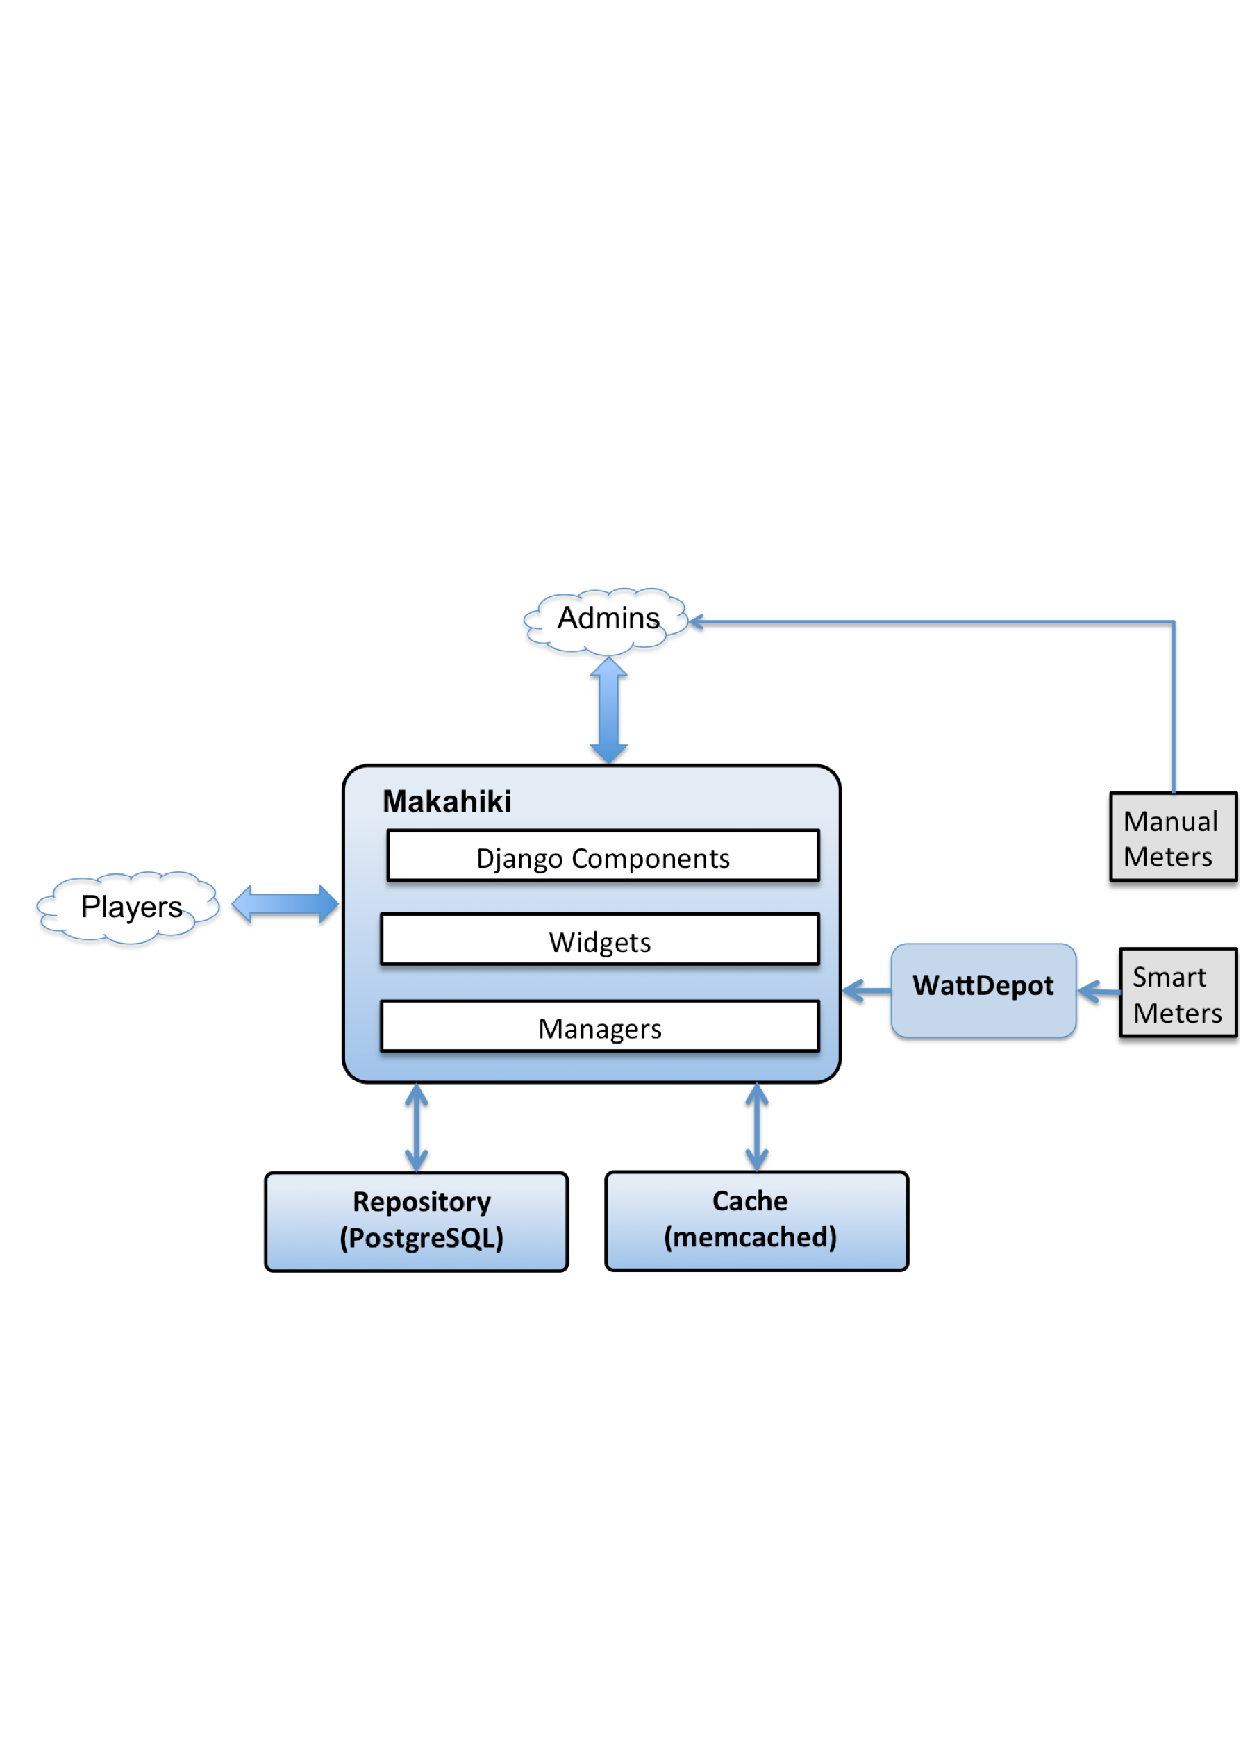
\epsfig{file=makahiki-system-architecture, width=3in}
\end{center}
\caption{Architecture of Makahiki}
\label{fig:makahiki-architecture}
\end{figure}

Makahiki consists of a configurable game engine that can be customized to the needs of different organizations.  It includes a library of pre-built game ``widgets'' that implement a variety of game mechanics.  Using the widgets, an organization can create a custom energy challenge in which players can compete individually and/or in teams to earn the most points by reducing their energy consumption as well as by learning about energy concepts in general.  Some of the pre-built widgets include:

\subsubsection{Smart Grid Game}

The {\em Smart Grid Game widget} shown in Figure \ref{fig:SmartGrid}, is the primary place players go to learn about energy issues and earn points. Actions are organized into a grid of squares (hence the name ``Smart Grid'') and organized by category columns. The grid contains four different types of actions: activities, commitments, events, and excursions.

\begin{figure}[ht!]
  \center
  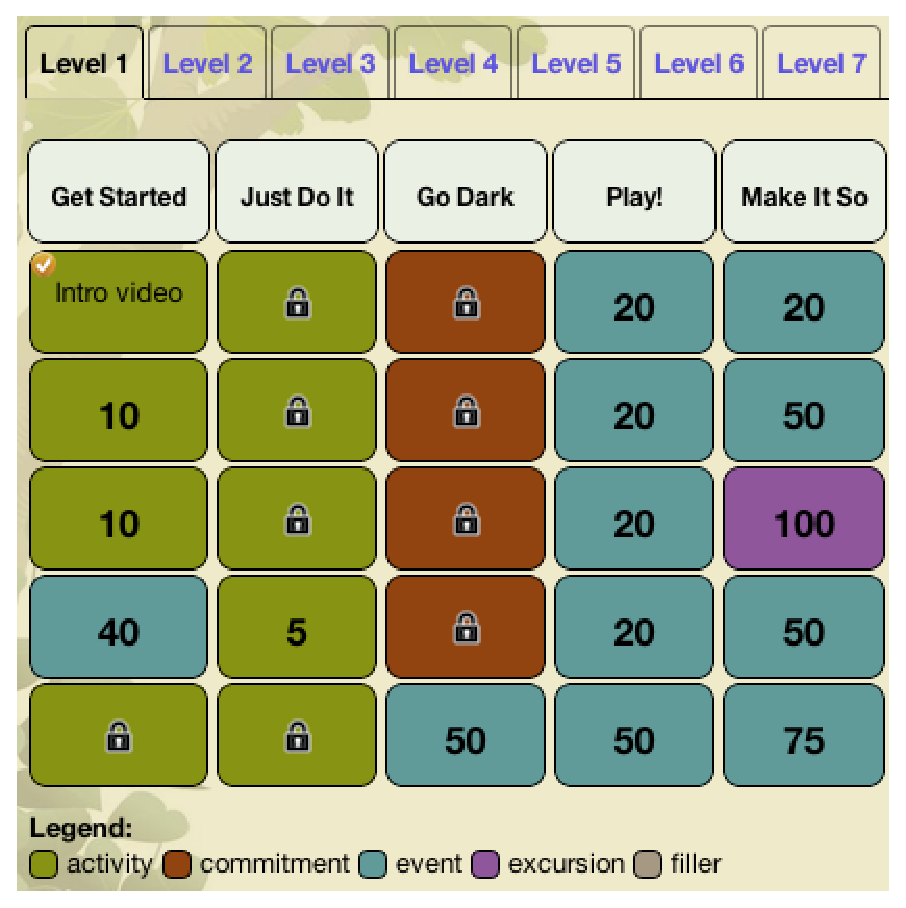
\includegraphics[width=0.4\textwidth]{smart-grid.eps}
  \caption{\em \small Smart Grid Game}
  \label{fig:SmartGrid}
\end{figure}

{\em Activities} are the most basic task available in the Smart Grid. In order to get points for an activity, a player will have to provide a response to the administrators. These responses can be a short textual answer or an uploaded picture. Administrators access a special admin section of the web application to approve or deny submissions. If a submission is approved, the player will receive the points for their submission. Otherwise, a player will be sent a website notification informing them that their submission was not approved, and a textual description by an administrator of why it was rejected. The player can change and resubmit their response and still earn the full point value for that task.

{\em Commitments} are pledges that the player will do something sustainable for a period of five days. Examples include: reducing shower time, taking the stairs, and turning off the lights when leaving a room. Because these commitments are not verifiable, they are worth fewer points than activities. Furthermore, a player can only have up to five active commitments at any given time. After the five day period is up, the player can then declare that they completed the commitment and immediately earn their points. They can then sign up for another commitment, including the one they just completed.

{\em Events and excursions} are tied to real world activities. Events are held on campus while excursions take place off campus. Seating is limited, so players are asked to sign up for events they wish to attend. Players that do so are provided with a 2 point signup bonus. Players can also set up a reminder that is sent to their email and/or their mobile phone before the event takes place. At the event, an administrator will hand out attendance codes printed on slips of paper that can be entered on the website. These attendance codes are generated by Makahiki and can only be used once. To discourage players from signing up and not attending, a 2 point penalty is assessed to players who do not submit an attendance code. If the player submits an attendance code for the event after receiving this penalty, the penalty is reversed.

Not all of the tasks in the Smart Grid Game are necessarily available at
the start of the game. We implemented a set of predicates that can be used to determine if a task is locked or unlocked for a player. These predicates include: completed a certain number of tasks within a category, completed all tasks within a category, completed certain tasks, and time-based unlocking (available after a certain date).

These predicates are implemented using a limited subset of Python and can
be changed within the Django admin interface. Competition designers can use
logical operators to combine any of these functions in order to organize
the players' path through the Smart Grid Game.

\subsubsection{Daily Energy Goal Game}

The {\em Daily Energy Goal Game widget} provides a way for players to earn points by reducing their current consumption from a baseline that is typically determined prior to the challenge. Both the historical baseline data and the current consumption is typically provided by API calls from Makahiki to an underlying WattDepot server.

\begin{figure}[t!]
  \center
  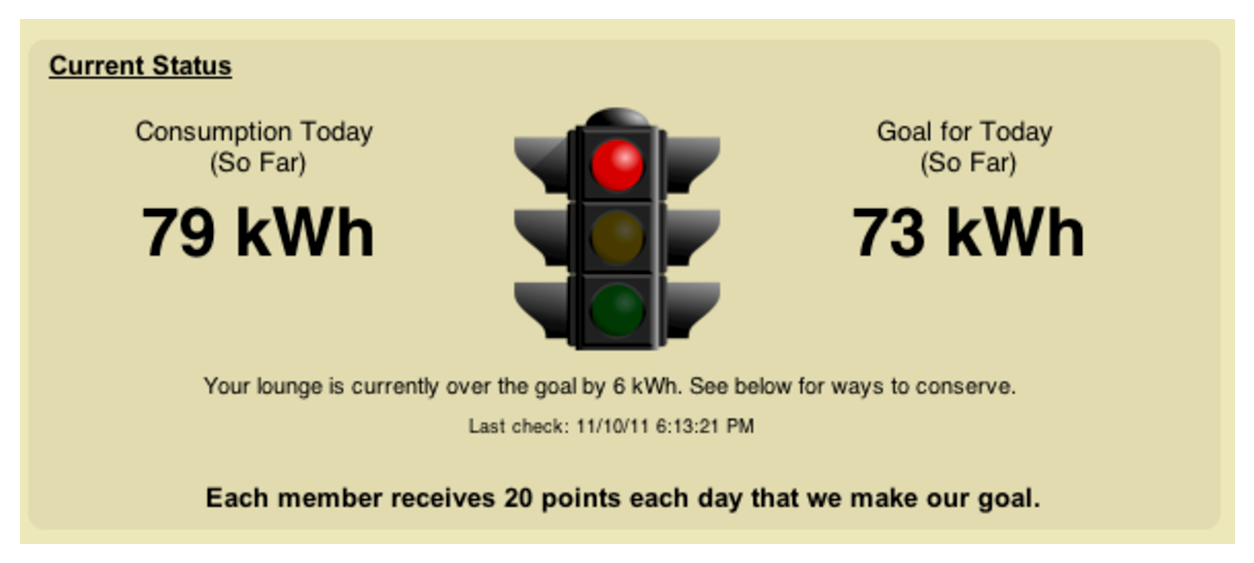
\includegraphics[width=0.4\textwidth]{daily-energy-goal-game.eps}
  \caption{\em \small Daily Energy Goal Game visualization}
  \label{fig:DailyEnergyGoal}
\end{figure}

The goal for each lounge is typically a percent reduction from their baseline usage of the previous two weeks. When a player goes to the energy page of the web application, they can view their lounge's current progress toward their daily energy goal. Near the end of the day, Makahiki checks the energy data from Wattdepot to see if a floor reached their goal. If the floor did reach their goal, each member of the floor that is participating in the game receives 20 points. The energy goal game provides a link between the energy conservation competition and the point competition.

Figure \ref{fig:DailyEnergyGoal} shows what a player would see when they go to the energy page. The Daily Energy Goal display shows both their current progress and their goal so far for two reasons. First, everyone will be under their actual energy goal for most of the day, so this display would not be very useful. Second, we have noticed that the students in the residence halls use more energy at night rather than during the day. Thus, it is easy to be under for most of the day and then jump over the goal at the very end. Displaying their goal so far provides a pace for players to follow.

\subsubsection{Raffle Game}

The {\em Raffle Game widget} provides a way to incentivize participation from all individuals, even those who are not in the running for a top prize. For every 25 points a player earns, they receive one virtual raffle ticket. Players can dynamically allocate their tickets to any raffle prizes they are interested in at any time, up to the end of the raffle.

\begin{figure}[t!]
  \center
  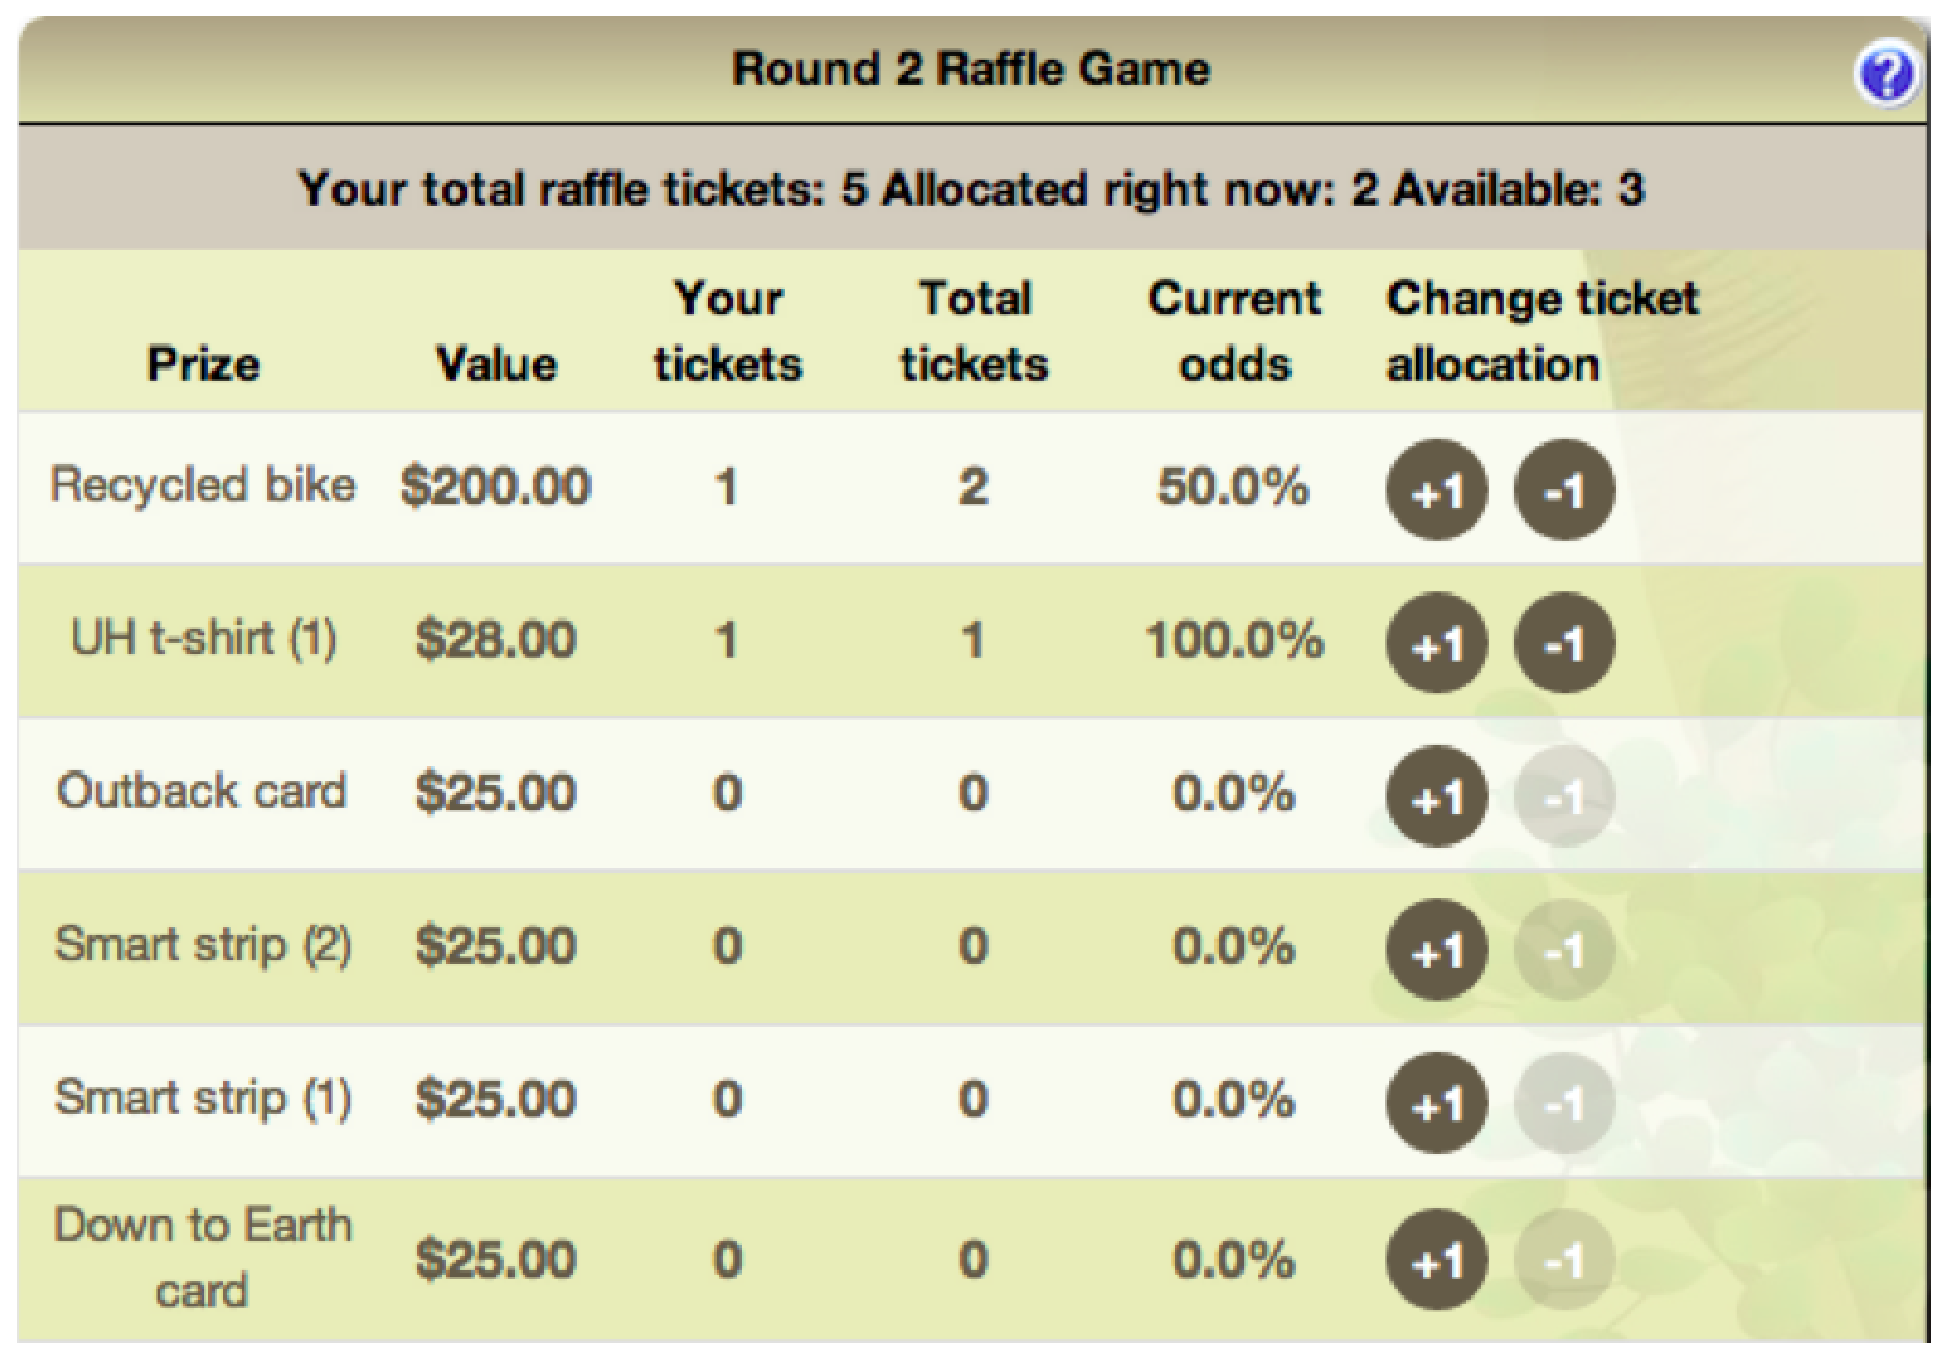
\includegraphics[width=0.4\textwidth]{raffle-small.eps}
  \caption{\em \small Raffle Game for the Overall Round}
  \label{fig:RaffleGame}
\end{figure}

Players can dynamically allocate their tickets to any raffle prizes they are interested in at any time, up to the end of the raffle. Each round of the competition has its own set of raffle prizes and any unused raffle tickets carry over to the next round. Raffle tickets are independent from a player's score; allocating a raffle ticket does not affect their rank. Figure \ref{fig:RaffleGame} shows an example of the Raffle Game.

\subsubsection{Social and Referral Bonuses}

The {\em Social and Referral Bonus widgets} provide game mechanics that help encourage participation by providing additional points to players who participate in activities with other players and/or facilitate the entry of new players into an energy challenge.

The social bonus is an administrator option when a task is created in the Smart Grid Game. It awards extra points if the player has done the task with someone else. Examples of tasks with social bonus include attending an event, recording a song related to energy, or measuring a shower water flow rate. When a player submits a response for a task with a social bonus, the player can provide the email address of the person who jointly completed the task. Once the other player completes the task, the social bonus is awarded. Social bonuses are not bi-directional; if the second player doesn't provide the first player's email address, only the first player will get the social bonus.

Players are led through a setup process when logging into Makahiki for the first time. One of the steps in this process is the referral bonus. If a player was referred by another player in the system, they can use this step to input their email address. Once the new player earns 30 points in the competition, both players are awarded a referral bonus of 10 points. Typically, going through the setup process gives you 25 points, so we wanted to encourage the new player to at least complete one additional task in order to get the referral bonus.

\subsubsection{Quest Engine}

One challenge we faced when designing Makahiki was providing adequate help to the player. The game needed to be intuitive, even if a new player coming to Makahiki has not participated in an energy competition. Unlike many web applications, such as webmail, Kukui Cup players do not know in advance what specific tasks they wish to accomplish. In an effort to provide a player with guidance through Makahiki after the setup process, we implemented the Quest Engine. Quests are used to guide the player through the various workflows of the site, like completing a task, signing up for an event, or allocating a raffle ticket. These quests can be created in the admin interface. They also use a set of predicates to determine unlock and completion conditions. These predicates are: participating in a task or type of task, completed a task or type of task, has a certain number of points (in a round or overall), completed a certain number of tasks in a category or of a given type, awarded a badge, wrote a post on their floor wall, and added a picture to their profile.

\subsubsection{Real Time Game Analytics}

Makahiki includes real-time game analytics that provides quantitative instrumentation to track when, where, and for how long each player accessed each page of the site and the interaction with each game components.  Unlike generic web server logs, this feature could track per-player game-specific behaviors in real-time. For example, instrumentation could enable us to determine how players allocated and deallocated tickets to the Raffle game, or whether they watched, paused, or skipped over the video portion of an Activity game. Figure \ref{fig:status} shows an example of the game analytics components.

\begin{figure}[t!]
  \center
  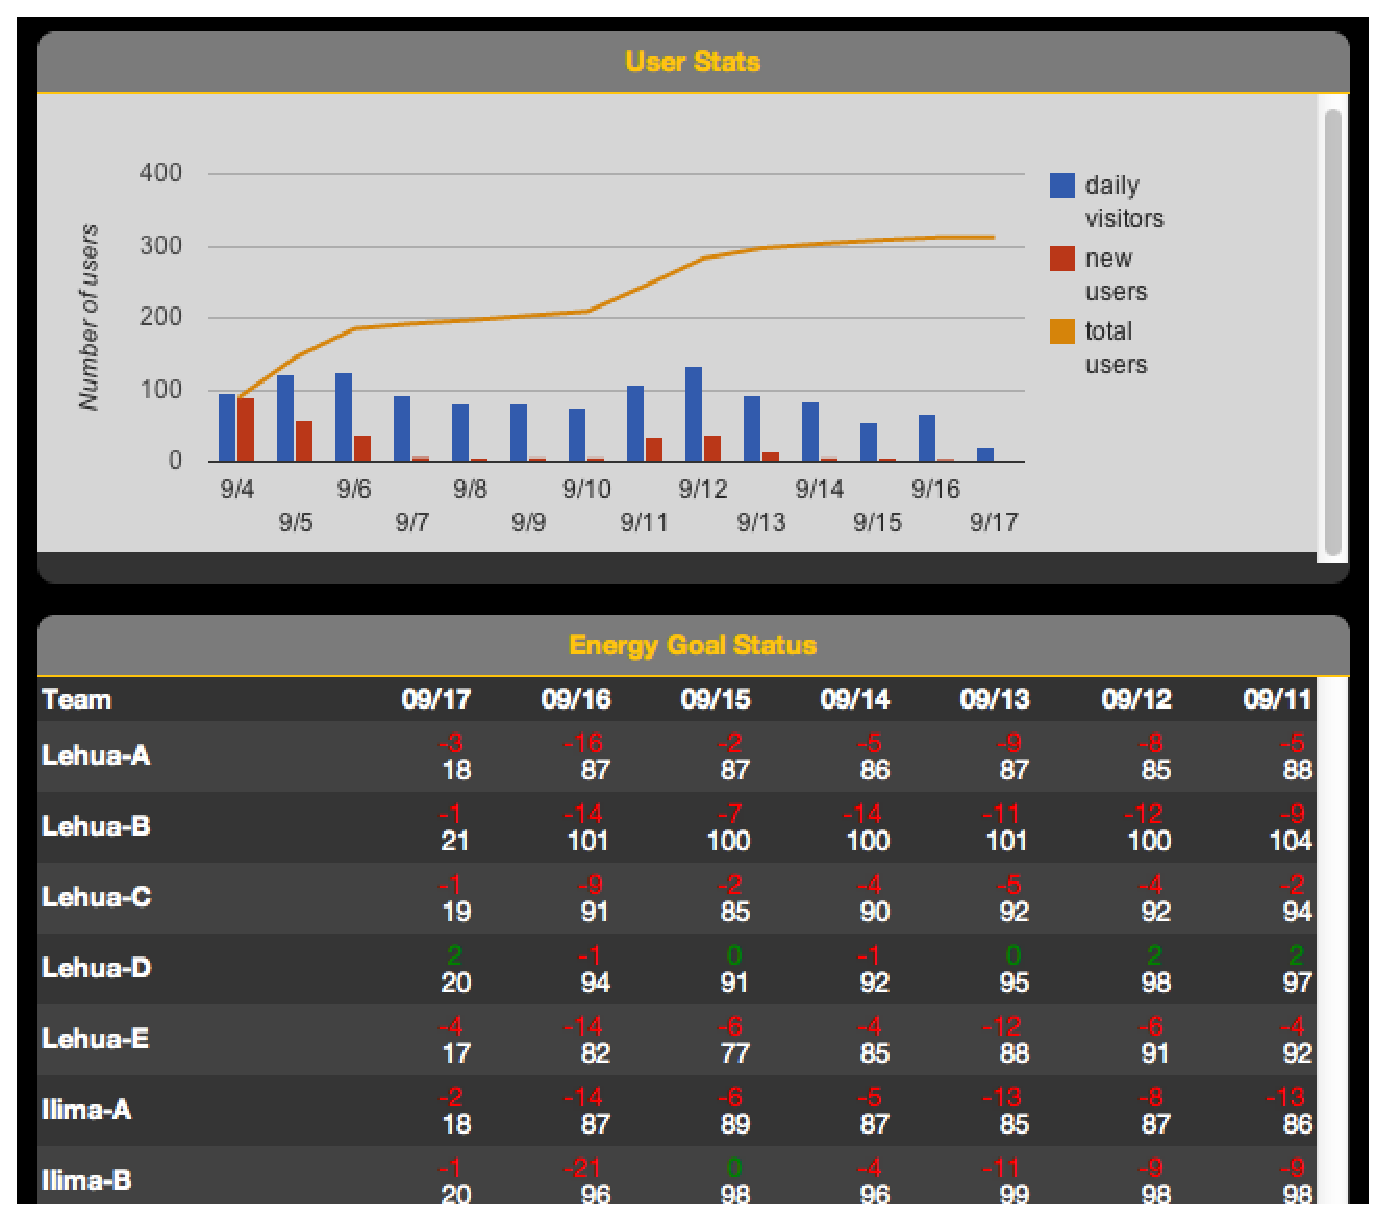
\includegraphics[width=0.4\textwidth]{status.eps}
  \caption{Real time game analytics}
  \label{fig:status}
\end{figure}

%\newpage
\section{Experiences}

To better understand the strengths and weaknesses of the Makahiki+WattDepot software stack, we have been designing and implementing an ``Energy Challenge'' called the Kukui Cup.  Development of the Kukui Cup challenge began in 2009, and the first Kukui Cup challenge was held in 2011 for over 1,000 first year students living in the residence halls at the University of Hawaii (UH) in Fall, 2011.  In Fall 2012, the second Kukui Cup challenge was held at the University of Hawaii using Makahiki+WattDepot.  In addition, Hawaii Pacific University (HPU) held a Kukui Cup challenge using Makahiki+WattDepot. Finally, an international organization called the East-West Center (EWC) held a Kukui Cup challenge using just Makahiki (their energy data was manually gathered by reading meters and entering the data by hand, so WattDepot was not needed for their challenge).    

The successful creation of four challenges by three different organizations over two years provides evidence that the software stack can be tailored to the differing needs of separate organizations.  First, UH uses meters by Electro-Industries Inc., while HPU uses meters by EGauge Inc., and EWC collected their energy data manually. Second, while UH and HPU challenges involved only energy consumption data, the EWC challenge involved both energy and water consumption data (which was also collected manually).  Third, the IT infrastructure at UH and HPU provided authentication services using CAS and LDAP, while EWC used the built-in Django authentication. Fourth, the user interface was customized to ``brand'' each challenge with the logo and other thematic elements of the sponsoring organization. 

On the other hand, it should be recognized that these organizations are in other ways quite similar: they are all institutions of post-secondary education, and they are all based in Hawaii.  These organizational similarities are mostly due to the desire by the 2012 challenges to reuse a significant amount of the content developed in 2011, which was oriented toward the Hawaii-based, college-aged demographic. For 2013 and beyond, we hope to expand our experiences with the software stack  ``downward'' into primary and secondary schools, and well as ``outward'' into residences and businesses. 

User response to the 2011 UH Kukui Cup challenge was positive, and provided evidence regarding the software stack's usability, functionality, and performance characteristics.   Over 400 students participated, for an adoption rate of approximately 40\%.  In a user survey conducted near the end of the challenge, over 90\% of users said they would participate in the challenge again if offered an opportunity.  60\%  said ``ease of use'' was the thing they liked best about the website.  40\% responded ``Nothing'' when asked what was confusing about the website, and 32\% responded ``Nothing'' when asked what they would change about the website.  The survey did yield insights into what could be improved, including the ability to introduce new games at points during the challenge, to provide better access to other player data, and to simplify navigation.  There was virtually no downtime during the 2011 challenge, and only one significant bug in the system (affecting scoring) was discovered during the challenge, which was fixed within a day of its discovery.  Finally, a pre- and post-challenge survey questionnaire yielded statistically significant evidence that participants in the challenge learned more about energy concepts than those not participating, demonstrating that the approach can serve to improve consumer knowledge of energy as needed for active engagement with the Smart Grid.

The 2012 challenges are ongoing as of the time of writing, so the following results must be viewed as preliminary, but our current experience is similarly positive to 2011.  The UH challenge participation rate so far appears to be slightly lower than last year, at about 33\%, though the HPU challenge participation rate so far is higher (approximately 50\%), and the EWC participation rate is much lower (around 6\%). None of the challenge instances have experienced significant downtime, and so far only 1 significant bug (affecting scoring) has been reported (and has again been fixed within a day).  Load testing of the software stack just prior to the 2012 challenge indicates a hypothetical throughput of around 200 concurrent users with acceptable page loading times, though we have not experienced that level of load in the current challenges. 

Our experiences over the past two years has provided many lessons learned, and some of the most important regarding the Makahiki+WattDepot software stack are:

{\em Collecting energy data is challenging.} As alluded to in our discussion of WattDepot, collecting accurate energy data requires significant planning and effort. The process of installing meters for the 2011 UH Kukui Cup started over one year before the meters were finally installed and ready for use, despite the cooperation and goodwill of all involved parties. Gaining an understanding of the electrical infrastructure of the residence halls proved crucial in the success of the UH Kukui Cup, as a renovation project led to the installation of additional distribution panels and thereby doubled the number of meters that were needed to measure electricity use. Due to delays in the installation of the meters for the 2011 UH Kukui Cup, a meter installation problem that led to inflated energy readings for one floor was not discovered until after the competition was complete and an energy audit of the building could be performed. Manual data collection also poses a variety of challenges. Existing meters for electricity and water may be configured for coarse monthly readings rather than the daily readings that are needed for a competition. Existing meters may also be installed in dirty or difficult to reach areas that make daily data collection unpleasant. If the challenge administrators wish to examine energy or water use after the challenge is complete, to determine if behavior changes made during the challenge are sustainable, daily manual data collection requires a long-term commitment. The lesson learned is for challenge administrators to start planning how they will obtain energy or water data as early as possible, since they are likely to encounter many challenges in collecting the data.

{\em Cloud-based hosting simplifies installation.}  During 2012, we have gained experience with both cloud-based hosting as well as local installation for the Makahiki+WattDepot software stack.  We have found that cloud-based hosting significantly simplifies the installation process and avoids certain types of installation-related bugs from occurring, particularly when system administrators are not familiar with the stack components that Makahiki+WattDepot depend upon (Django, Java, Python, git, etc.)  On the other hand, cloud-based hosting incurs costs (in our experience, between \$50-\$100/month for these challenges) and may incur constraints (for example, the Heroku hosting platform currently has minimal support for LDAP authentication).  The Makahiki Manual \cite{MakahikiManual} provides instructions for both cloud-based and local installation, providing some idea of the differences between the two approaches.  The lesson learned is to use cloud-based hosting when possible, or allow plenty of time for administrators to work through the software stack installation issues. Makahiki+WattDepot is not yet a ``plug-and-play'' system.

{\em Challenge design and administration is time consuming.} Despite the freely providing the Makahiki+WattDepot software stack to HPU and EWC, along with content developed specifically for college-age residents of Hawaii, the administrators still expressed surprise at the how time consuming it was to design and administrate the running of their respective challenges.  This appears to be due to the fact that the software stack enables a variety of game mechanics (such as the Smart Grid Game, Raffle Game, Badges, and point-based Prizes) not present in more simplistic energy challenges.  For example, the Smart Grid Game requires configuration of the widget including what activities to include and when/where they appear in the game.  The Raffle Game and point-based awards requires the collection of appropriate prizes. While we provided a library of almost 100 activities from 2011, all of the 2012 challenges required the definition of at least a few new events.  Thus, although the result is a more sophisticated experience for the participants, the up front design and overhead during execution was generally surprising to the administrators. The Kukui Cup Challenge Planning Guide \cite{KukuiCupChallengePlanningGuide} provides more details on this process.  The lesson learned is to make sure that potential organizational sponsors understand that the use of this software technology is not intended to make it more simple for them to run an energy challenge, but rather to enable them to create a more sophisticated energy challenge than would otherwise be possible.

{\em Scalability cuts across both design and implementation.}  So far, the use of the Makahiki+WattDepot software stack has been limited to relatively small user communities of 1,000 participants or less.  We believe that the system and approach would scale relatively well to some small number of multiples of that number, say to a maximum of 10,000 challenge participants.  On the other hand, there are both design and implementation challenges in scaling the software stack to communities of significantly larger than 10,000 participants.

On the design side, Makahiki currently requires administrators to approve each submission by a participant in order for that participant to receive points.   In the UH challenges, that results in administrative approval of around 4,000 individual submissions over the course of the challenge.  This incurs administrative overhead, but makes it easier to verify that players are actually taking part in activities and improves the sense of fairness in the game.  On the other hand, we do not believe this approach would be practical if there were an order of magnitude more submissions to process.  To scale, the current manual approval process must be automated, and must be done in a manner that preserves essential game mechanics.  For example, simply changing the current short answer verification format by multiple choice could result is players just randomly selecting values until they find the right one.  Multiple choice also does not support certain types of activities where the submission is a link, a photo, or even a poem.  So, scaling up by an order of magnitude might affect the types of activities that can be supported in the challenge. Peer review of action submissions is one possible solution, but would require careful design and testing to ensure the competitive nature of the challenge does not encourage unfair evaluation of submissions.

On the implementation side, our current performance testing indicates a maximal throughput of approximately 200 concurrent users.  Interestingly, increasing the number of server/web resources available through cloud-based hosting does not appear to appreciably increase maximal throughput.  Thus, it does not appear to be true that cloud-based hosting will magically ``solve'' the scalability problem for the Makahiki+WattDepot software stack.  Because the current level of throughput is adequate for the communities we are current targeting, we have not investigated this issue further.  The lesson learned is that if an organization wants to perform an energy challenge for a community of more than 10,000 users, significant design and implementation challenges must be addressed.


\section{Conclusions/Future Directions}

Our experiences thus far with the Makahiki+WattDepot software stack have shown it to be a
reliable and performant system for the provision of sophisticated energy challenges to
address the need for informed consumers in the development of the Smart Grid.

One future direction involves the development of a consortium of local organizations in
order to explore the use of this software stack in new settings.  This will create
challenges at both the design and implementation levels.   Moving outside of the context
of either Hawaii or college-aged users will necessitate development of significant new
forms of content, including activities, workshops, events, and videos. This challenge,
while significant, does not necessitate significant changes to the Makahiki+WattDepot
software stack.

A far more challenging future direction is an island-wide Kukui Cup, in which all of the residents of
Oahu would be able to login to the system and play the game. This creates challenges on
multiple levels: providing content appropriate to the user (an elementary student should
have activities different from her mother and father), obtaining energy data for
residential users from the local utility in a manner appropriate for the challenge and
interface this data with the system, and finally resolving the scalability problem
identified in the last section.  We will require the engagement of multiple stakeholders
from across the community spectrum to identify and resolve these issues. 





%ACKNOWLEDGMENTS are optional
\section{Acknowledgments}

Add acknowlegements to sponsors and other KC team members.

% The following two commands are all you need in the
% initial runs of your .tex file to
% produce the bibliography for the citations in your paper.
\bibliographystyle{abbrv}
\bibliography{smartconsumer,csdl-trs,gamification,sustainability}
\balancecolumns

\end{document}
